\documentclass{standalone}
\usepackage{textcomp}
\usepackage{pgfplots}
\begin{document}
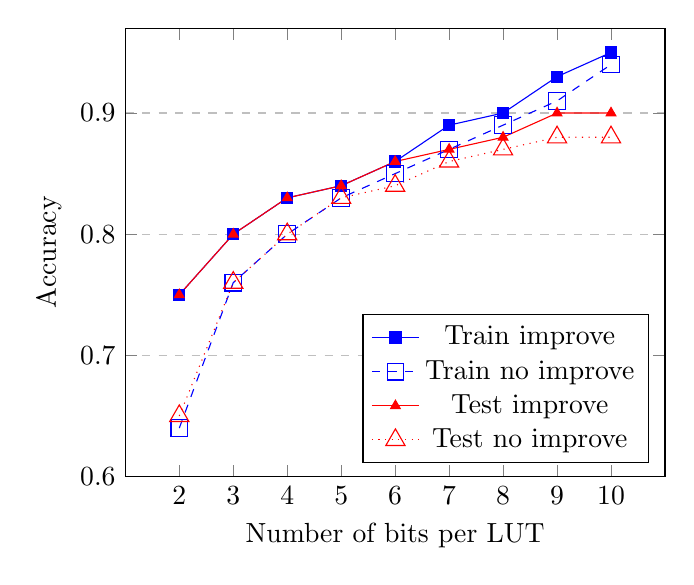
\begin{tikzpicture}
\begin{axis}[
    %title={Real data},
    xlabel={Number of bits per LUT},
    ylabel={Accuracy},
    xmin=1, xmax=11,
    ymin=0.6, ymax=0.97,
    xtick={2,3,4,5,6,7,8,9,10},
    ytick={0.5,0.6,0.7,0.8,0.9,1.00},
    legend pos=south east,
    ymajorgrids=true,
    grid style=dashed,
]

\addplot[
    color=blue,
    mark=square*,
    ]
    coordinates {
    (2,0.75)(3,0.80)(4,0.83)(5,0.84)(6,0.86)(7,0.89)(8,0.90)(9,0.93)(10,0.95)
    };
    \addlegendentry{Train improve}

\addplot[
    color=blue,
    mark=square,
    mark options={solid, scale=1.5},
    dashed,
    ]
    coordinates {
    (2,0.64)(3,0.76)(4,0.8)(5,0.83)(6,0.85)(7,0.87)(8,0.89)(9,0.91)(10,0.94)
    };
    \addlegendentry{Train no improve}

\addplot[
    color=red,
    mark=triangle*,
    ]
    coordinates {
    (2,0.75)(3,0.80)(4,0.83)(5,0.84)(6,0.86)(7,0.87)(8,0.88)(9,0.90)(10,0.90)
    };
    \addlegendentry{Test improve}

\addplot[
    color=red,
    mark=triangle,
    mark options={solid, scale=2},
    dotted,
    ]
    coordinates {
    (2,0.65)(3,0.76)(4,0.8)(5,0.83)(6,0.84)(7,0.86)(8,0.87)(9,0.88)(10,0.88)
    };
    \addlegendentry{Test no improve}

\end{axis}
\end{tikzpicture}
\end{document}
